% Generated by jats2tex@0.11.1.0
\documentclass{article}
\usepackage[T1]{fontenc}
\usepackage[utf8]{inputenc} %% *
\usepackage[portuges,spanish,english,german,italian,russian]{babel} %% *
\usepackage{amstext}
\usepackage{authblk}
\usepackage{unicode-math}
\usepackage{multirow}
\usepackage{graphicx}
\usepackage{etoolbox}
\usepackage{xtab}
\usepackage{enumerate}
\usepackage{hyperref}
\usepackage{penalidades}
\usepackage[footnotesize,bf,hang]{caption}
\usepackage[nodayofweek,level]{datetime}
\usepackage[top=0.85in,left=2.75in,footskip=0.75in]{geometry}
\newlength\savedwidth
\newcommand\thickcline[1]{\noalign{\global
\savedwidth
\arrayrulewidth
\global\arrayrulewidth 2pt}
\cline{#1}
\noalign{\vskip\arrayrulewidth}
\noalign{\global\arrayrulewidth\savedwidth}}
\newcommand\thickhline{\noalign{\global
\savedwidth\arrayrulewidth
\global\arrayrulewidth 2pt}
\hline
\noalign{\global\arrayrulewidth\savedwidth}}
\usepackage{lastpage,fancyhdr}
\usepackage{epstopdf}
\pagestyle{myheadings}
\pagestyle{fancy}
\fancyhf{}
\setlength{\headheight}{27.023pt}
\lhead{
\includegraphics[width=10mm]{logo.png}}
\rhead{\ifdef{\journaltitle}{\journaltitle}{}
\ifdef{\volume}{vol.\,\volume}{}
\ifdef{\issue}{(\issue)}{}
\ifdef{\fpage}{\fpage--\lpage\,pp.}}
\rfoot{\thepage/\pageref{LastPage}}
\renewcommand{\footrule}{\hrule height 2pt \vspace{2mm}}
\fancyheadoffset[L]{2.25in}
\fancyfootoffset[L]{2.25in}
\lfoot{\sf \ifdef{\articledoi}{\articledoi}{}}
\setmainfont{Linux Libertine O}
\renewcommand*{\thefootnote}{\alph{footnote}}
\makeatletter
\newcommand{\fn}{\afterassignment\fn@aux\count0=}
\newcommand{\fn@aux}{\csname fn\the\count0\endcsname}
\makeatother

\newcommand{\journalid}{Rev Saude Publica}
\newcommand{\journaltitle}{Revista de Saúde Pública}
\newcommand{\abbrevjournaltitle}{Rev. Saúde Pública}
\newcommand{\issnppub}{0034-8910}
\newcommand{\issnepub}{1518-8787}
\newcommand{\publishername}{Faculdade de Saúde Pública da Universidade de São
Paulo}
\newcommand\articledoi{\textsc{doi} 10.1590/S0034-8910.2014048004540}
\def\subject{Artigos Originais}\newcommand{\subtitlestyle}[1]{--
\emph{#1}\medskip}
\newcommand{\transtitlestyle}[1]{\par\medskip\Large #1}
\newcommand{\transsubtitlestyle}[1]{-- \Large\emph{ #1}}

\newcommand{\titlegroup}{
\ifdef{\subtitle}{\subtitlestyle{\subtitle}}{}
\ifdef{\transtitle}{\transtitlestyle{\transtitle}}{}
\ifdef{\transsubtitle}{\transsubtitlestyle{\transsubtitle}}{}}

\title{Sorteio intradomiciliar em inquéritos de saúde\titlegroup{}}
\newcommand{\transtitle}{Sorteo intra-domiciliar en pesquisa de salud}
\author[{I}]{Alves, Maria Cecilia Goi Porto}
\author[{I}]{Escuder, Maria Mercedes Loureiro}
\author[{II}]{Claro, Rafael Moreira}
\author[{\textsc{iii}}]{Silva, Nilza Nunes da}
\affil[i]{Secretaria de Estado da Saúde de São Paulo}
\affil[ii]{Universidade Federal de Minas Gerais}
\affil[iii]{Universidade de São Paulo}
\def\authornotes{Correspondência | Correspondence: Maria Cecilia Goi Porto
Alves. Rua Santo Antônio, 590. 01314-000 São Paulo, SP, Brasil. E-mail:
cecilia@isaude.sp.gov.br
Os autores declaram não haver conflito de interesses.}
\date{ 02 2014}
\def\volume{48}
\def\issue{1}
\def\fpage{86}
\def\lpage{93}
\def\permissions{This is an Open Access article distributed under the terms of
the Creative Commons Attribution Non-Commercial License, which permits
unrestricted non-commercial use, distribution, and reproduction in any medium,
provided the original work is properly cited.}
\newcommand{\kwdgroup}{Inquéritos Epidemiológicos, métodos, Inquéritos
Demográficos, Amostragem por Conglomerados, Amostragem}
\newcommand{\kwdgroupes}{Encuestas Epidemiológicas, métodos, Encuestas
Demográficas, Muestreo por Conglomerados, Muestreo}
%%% Nota %%%%%%%%%%%%%%%%%%%%%%%%%%%%%%%%%%%%%%%%%%%%%%%%%%%%%%%%
\expandafter\newcommand\csname \endcsname{
Trabalho apresentado no \textsc{viii} Congresso de Epidemiologia, São Paulo, SP, 2011 e
na \textsc{iii} Escola de Amostragem e Metodologia de Pesquisa, Juiz de Fora, MG, 2011.}
%%% Nota fn1 %%%%%%%%%%%%%%%%%%%%%%%%%%%%%%%%%%%%%%%%%%%%%%%%%%%%%%%%
\expandafter\newcommand\csname fn1\endcsname{
Instituto Brasileiro de Geografia e Estatística (BR). Pesquisa Nacional por
Amostra de Domicílios. Brasília (DF); [s.d.].}
%%% Nota fn2 %%%%%%%%%%%%%%%%%%%%%%%%%%%%%%%%%%%%%%%%%%%%%%%%%%%%%%%%
\expandafter\newcommand\csname fn2\endcsname{
Centers for Disease Control and Prevention (US). National Health Interview
Survey. Washington (DC); [s.d.].}
%%% Nota fn3 %%%%%%%%%%%%%%%%%%%%%%%%%%%%%%%%%%%%%%%%%%%%%%%%%%%%%%%%
\expandafter\newcommand\csname fn3\endcsname{
National Centre for Social Research (UK). Health Survey for England. Londres;
[s.d.].}
%%% Nota fn4 %%%%%%%%%%%%%%%%%%%%%%%%%%%%%%%%%%%%%%%%%%%%%%%%%%%%%%%%
\expandafter\newcommand\csname fn4\endcsname{
Fundação Oswaldo Cruz (BR). Pesquisa Mundial de Saúde no Brasil. Rio de Janeiro;
[s.d.].}
%%% Nota fn5 %%%%%%%%%%%%%%%%%%%%%%%%%%%%%%%%%%%%%%%%%%%%%%%%%%%%%%%%
\expandafter\newcommand\csname fn5\endcsname{
Centers for Disease Control and Prevention (US). National Health and Nutrition
Examination. Washington (DC); [s.d.].}
%%% Nota fn6 %%%%%%%%%%%%%%%%%%%%%%%%%%%%%%%%%%%%%%%%%%%%%%%%%%%%%%%%
\expandafter\newcommand\csname fn6\endcsname{
Institut de Veille Sanitaire (FR). Etude Nationale Nutrition Santé. Paris ;
[s.d.].}
%%% Nota fn7 %%%%%%%%%%%%%%%%%%%%%%%%%%%%%%%%%%%%%%%%%%%%%%%%%%%%%%%%
\expandafter\newcommand\csname fn7\endcsname{
Statistics Canadá (CA). Canadian Community Health Survey. Ottawa; [s.d.].}
%%% Nota fn8 %%%%%%%%%%%%%%%%%%%%%%%%%%%%%%%%%%%%%%%%%%%%%%%%%%%%%%%%
\expandafter\newcommand\csname fn8\endcsname{
Alves \textsc{mcgp}, Escuder \textsc{mml}. Plano de amostragem. In. Escuder \textsc{mml}, Monteiro \textsc{phn},
Pupo LR. Acesso aos serviços de saúde em municípios da baixada santista. São
Paulo: Instituto de saúde; 2009. (Temas em saúde coletiva, 8).}
%%% Nota fn9 %%%%%%%%%%%%%%%%%%%%%%%%%%%%%%%%%%%%%%%%%%%%%%%%%%%%%%%%
\expandafter\newcommand\csname fn9\endcsname{
Escuder \textsc{mml}, Monteiro \textsc{phn}, Pupo LR. Acesso aos serviços de saúde em municípios
da baixada santista. São Paulo: Instituto de saúde; 2009. (Temas em saúde
coletiva, 8).}
%%% Nota %%%%%%%%%%%%%%%%%%%%%%%%%%%%%%%%%%%%%%%%%%%%%%%%%%%%%%%%
\expandafter\newcommand\csname \endcsname{
Trabalho financiado pelo Projeto de Expansão e Consolidação do Programa da Saúde
da Família – \textsc{proesf} 2006 do Ministério da Saúde.}

\begin{document}
\selectlanguage{portuges}
\section*{Metadados não aplicados}
\begin{itemize}
\item[\textbf{língua do artigo}]{Português}
\ifdef{\journalid}{\item[\textbf{journalid}] \journalid}{}
\ifdef{\journaltitle}{\item[\textbf{journaltitle}] \journaltitle}{}

\ifdef{\journalsubtitle}{\item[\textbf{journalsubtitle}] \journaltitle}{}
\ifdef{\transjournaltitle}{\item[\textbf{journaltitle}] \journaltitle}{}
\ifdef{\transjournalsubtitle}{\item[\textbf{journalsubtitle}] \journaltitle}{}

\ifdef{\abbrevjournaltitle}{\item[\textbf{abbrevjournaltitle}]
\abbrevjournaltitle}{}
\ifdef{\issnppub}{\item[\textbf{issnppub}] \issnppub}{}
\ifdef{\issnepub}{\item[\textbf{issnepub}] \issnepub}{}
\ifdef{\publishername}{\item[\textbf{publishername}] \publishername}{}
\ifdef{\publisherid}{\item[\textbf{publisherid}] \publisherid}{}
\ifdef{\subject}{\item[\textbf{subject}] \subject}{}
\ifdef{\transtitle}{\item[\textbf{transtitle}] \transtitle}{}
\ifdef{\authornotes}{\item[\textbf{authornotes}] \authornotes}{}
\ifdef{\articleid}{\item[\textbf{articleid}] \articleid}{}
\ifdef{\articledoi}{\item[\textbf{articledoi}] \articledoi}{}
\ifdef{\volume}{\item[\textbf{volume}] \volume}{}
\ifdef{\issue}{\item[\textbf{issue}] \issue}{}
\ifdef{\fpage}{\item[\textbf{fpage}] \fpage}{}
\ifdef{\lpage}{\item[\textbf{lpage}] \lpage}{}
\ifdef{\permissions}{\item[\textbf{permissions}] \permissions}{}
\end{itemize}
\maketitle

\begingroup

\begin{abstract}
\section{\textsc{objetivo}}

: Comparar a eficiência e a acurácia de delineamentos de amostragem com e sem
sorteio intradomiciliar em inquéritos de saúde.

\section{\textsc{métodos}}

: Com base nos dados de um inquérito realizado na Baixada Santista, SP, entre
2006 e 2007, foram retiradas 1.000 amostras sob cada um dos delineamentos e, em
cada amostra, foram obtidas estimativas para pessoas de 18 a 59 anos de idade e
de 18 anos e mais. Sob o primeiro, foram sorteados 40 setores censitários, 12
domicílios por setor e uma pessoa por domicílio. Na análise, os dados foram
ponderados pelo número de adultos residentes nos domicílios. Sob o segundo,
foram sorteados 40 setores, seis domicílios por setor para o grupo de 18 a 59
anos de idade e cinco ou seis domicílios para o grupo de 18 anos e mais. Não
houve sorteio dentro do domicílio. Medidas de precisão e de vício das
estimativas de proporção para 11 indicadores foram calculadas nos dois conjuntos
finais das amostras selecionadas para os dois tipos de delineamentos. Estes
foram comparados por meio das medidas relativas: coeficiente de variação, razão
vício/média, razão vício/erro padrão e erro quadrático médio relativo. O custo
foi comparado considerando custo básico por pessoa, custo por domicílio e
números de pessoas e domicílios.

\section{\textsc{resultados}}

: Os vícios mostraram-se desprezíveis nos dois delineamentos. A precisão foi
maior para o delineamento sem sorteio e o custo foi menor.

\section{\textsc{conclusões}}

: O delineamento sem sorteio intradomicilar mostrou-se superior em termos de
eficiência e acurácia, devendo ser a opção preferencial do pesquisador. O
sorteio de moradores deve ser adotado quando houver razões referentes ao objeto
de estudo que possam levar à introdução de vícios nas respostas dos
entrevistados no caso de vários moradores responderem ao questionário proposto.

\iflanguage{portuges}{\medskip\noindent\textbf{Palavras-chave:} \kwdgroup}{}
\iflanguage{english}{\medskip\noindent\textbf{Keywords:} \kwdgroupen}{}
\iflanguage{spanish}{\medskip\noindent\textbf{Palavras claves:} \kwdgroupes}{}
\iflanguage{french}{\medskip\noindent\textbf{Mots clés:} \kwdgroupfr}{}
\end{abstract}
\endgroup

\begingroup
\renewcommand{\section}[1]{\subsection*{#1}}
\begin{otherlanguage}{spanish}

\begin{abstract}

\textsc{objetivo}: Comparar la eficiencia y la precisión de delineamientos de muestreo
con y sin sorteo intra-domiciliar en pesquisas de salud.

\textsc{métodos}: Con base en los datos de una pesquisa realizada en la Baixada Santista,
SP – Brasil, entre 2006 y 2007, se retiraron 1.000 muestras considerando cada
uno de los delineamientos y, en cada muestra, se obtuvo estimativas para
personas de 18 a 59 años de edad y de 18 años y más. En el primero, fueron
sorteados 40 sectores censados, 12 domicilios por sector y una persona por
domicilio. En el análisis, los datos fueron ponderados por el número de adultos
residentes en los domicilios. En el segundo, se sortearon 40 sectores, seis
domicilios por sector para el grupo de 18 a 59 años de edad y cinco o seis
domicilios para el grupo de 18 años y más. No hubo sorteo dentro del domicilio.
Medidas de precisión y de vicio de las estimativas de proporción para 11
indicadores fueron calculadas en los dos conjuntos finales de muestras
seleccionadas para los dos tipos de delineamientos. Ambos fueron comparados por
medio de medidas relativas: coeficiente de variación, cociente vicio/promedio,
cociente vicio/desviación estándar y desviación media cuadrática relativa. El
costo fue comparado considerando costo básico por persona, costo por domicilio y
número de personas y domicilios.

\textsc{resultados}: Los vicios se mostraron insignificantes en los dos delineamientos.
La precisión fue mayor para el delineamiento sin sorteo y el costo fue menor.

\textsc{conclusiones}: El delineamiento sin sorteo intra-domiciliar se mostró superior en
términos de eficiencia y precisión, siendo la opción preferencial del
investigador. El sorteo de la población debe ser adoptado cuando existan motivos
relacionados con el objeto de estudio que puedan llevar a la introducción de
vicios en las respuestas de los entrevistados en el caso de que varios de ellos
respondan al cuestionario propuesto.

\ifdef{\kwdgroupes}{\medskip\noindent\textbf{Palavras claves:} \kwdgroupes}{}
\end{abstract}
\end{otherlanguage}
\endgroup
\section{\textsc{introdução}}

Em inquéritos de base populacional em que amostras em múltiplos estágios são
retiradas, o domicílio é sempre utilizado como unidade de amostragem em algum
desses estágios. Considerando que as pessoas são os elementos de interesse de
tais inquéritos, o domicílio deve ser visto como um conglomerado, na medida em
que engloba ou pode englobar vários elementos.

Há, portanto, duas opções para os delineamentos de amostragem a serem
utilizados: considerar o domicílio como unidade de último estágio e incluir na
amostra todos os moradores que preencham os critérios
estabelecidos\footnote{\fn1}\textsuperscript{,}\footnote{\fn2}\textsuperscript{,}\footnote{\fn3}
ou considerar a inclusão no delineamento de mais um estágio de seleção e sortear
um ou mais moradores de cada domicílio.\footnote{\fn4}\textsuperscript{,}\footnote{\fn5}\textsuperscript{,}\footnote{\fn6}\textsuperscript{,}\footnote{\fn7}

O primeiro deles é o mais frequentemente
utilizado\textsuperscript{[}\textsuperscript{4}\textsuperscript{]}
e tem como principal vantagem a possibilidade, em função da ausência de sorteio
intradomiciliar, de manter a equiprobabilidade de amostras que tenham sido
originalmente concebidas com essa propriedade. Por outro lado, entrevistar
várias pessoas de uma mesma família poderia diminuir a precisão das estimativas
como consequência da homogeneidade existente dentro dos domicílios.

Com o sorteio intradomiciliar e a consequente inclusão na amostra de um número
maior de domicílios, esse problema seria contornado. Haveria necessidade, no
entanto, de utilizar pesos de amostragem para compensar as diferentes
probabilidades de seleção, o que também acarretaria uma diminuição da precisão
das estimativas.

O sorteio de pessoas no domicílio é o procedimento mais adequado quando questões
sensíveis estão presentes nos questionários e supõe-se que as respostas de um
entrevistado podem influenciar as de outros membros da
família.\textsuperscript{[}\textsuperscript{5}\textsuperscript{]}
Tem sido adotado, ainda, em algumas pesquisas nas quais o questionário é
excessivamente longo, acreditando-se que as taxas de resposta poderiam ser
afetadas se a entrevista for percebida como onerosa pelos
respondentes.\textsuperscript{[}\textsuperscript{5}\textsuperscript{]}
Nesses casos, os sorteios são usualmente realizados utilizando procedimentos
propostos por Kish, adaptados ou não,\textsuperscript{[}\textsuperscript{2}\textsuperscript{]}\textsuperscript{,}\textsuperscript{[}\textsuperscript{9}\textsuperscript{]}
ou com base em técnicas que selecionam os indivíduos a partir de suas datas de
aniversários.\textsuperscript{[}\textsuperscript{13}\textsuperscript{]}\textsuperscript{,}\textsuperscript{[}\textsuperscript{14}\textsuperscript{]}\textsuperscript{,}\textsuperscript{[}\textsuperscript{16}\textsuperscript{]}

Há pouca literatura sobre sorteio intradomiciliar. Faltam estudos que discutam
quantas pessoas devem ser selecionadas nos domicílios e o impacto das diversas
alternativas disponíveis nas estatísticas produzidas.

O objetivo deste estudo foi comparar a eficiência e a acurácia de delineamentos
de amostragem sem sorteio intradomiciliar e com sorteio de uma única pessoa.

\section{\textsc{métodos}}

Tomou-se como ponto de partida o inquérito domiciliar sobre acesso a serviços de
saúde da Baixada Santista, SP, realizado entre 2006 e 2007, no qual haviam sido
realizadas 6.826 entrevistas em 2.189 domicílios de 100 setores censitários,
incluindo-se na amostra todas as pessoas residentes nos domicílios
sorteados.\footnote{\fn8}

O tamanho dessa amostra e a inclusão de todas as pessoas dos domicílios, com
exceção dos que se recusaram a participar do inquérito, permitiram que ela fosse
a população de estudo deste trabalho. Dessa forma, do conjunto de dados do
inquérito, foram sorteadas 1.000 amostras sob cada um dos delineamentos em
avaliação, com e sem sorteio intradomiciliar. Em cada amostra, foram obtidas
estimativas para dois grupos populacionais: o de adultos (18 a 59 anos de idade)
e o de adultos e idosos em conjunto (18 anos e mais). Esses grupos foram
escolhidos por constituírem, com frequência, populações alvo de inquéritos de
saúde.

O primeiro delineamento considerou três estágios de seleção: setor censitário,
domicílio e indivíduo. Foram sorteados 40 setores censitários com probabilidade
proporcional ao tamanho e, posteriormente, 12 domicílios por setor e uma pessoa
por domicílio. O tamanho planejado da amostra foi de 480 pessoas. Para compensar
as diferenças nas probabilidades de seleção, foram introduzidos pesos
equivalentes aos números de adultos ou adultos e idosos existentes nos
domicílios selecionados.

O segundo delineamento considerou dois estágios de seleção: setor censitário e
domicílio. Foram também sorteados 40 setores censitários com probabilidade
proporcional ao tamanho e seis domicílios por setor para adultos e cinco ou seis
domicílios (média de 5,66) para adultos e idosos. Não houve sorteio dentro do
domicílio. Todas as pessoas dos grupos populacionais de interesse residentes nos
domicílios sorteados foram entrevistadas. Considerando, respectivamente, razões
de dois adultos e de 2,12 adultos e idosos por domicílio, esperava-se alcançar
480 entrevistas em cada amostra.

O aplicativo Stata Versão 11.2 foi empregado para a produção de uma estrutura de
\textit{looping}
capaz de produzir as 1.000 amostras utilizadas em cada um dos delineamentos em
avaliação. A função \textit{runiform}
foi utilizada para o estabelecimento de um ponto aleatório para início do
sorteio dos setores e, a seguir, dos domicílios. O comando \textit{sample}
foi utilizado para a seleção aleatória do morador dentro de cada um dos
domicílios nos delineamentos com sorteio intradomiciliar.

As frações de amostragem utilizadas no sorteio das amostras e outros aspectos
referentes aos planos de amostragem estão apresentados na Tabela 1.

Tabela 1Aspectos referentes aos delineamentos de amostragem. Região
Metropolitana da Baixada Santista, SP, 2006-2007.0034-8910-rsp-48-01-0086-gt01

Para a obtenção das estimativas utilizadas, foram escolhidos 11 indicadores de
saúde do Inquérito Domiciliar sobre Acesso a Serviços de Saúde da Baixada
Santista,\footnote{\fn9}
agrupados em três categorias, a saber: 1. Situação de saúde (auto avaliação de
saúde como ruim ou péssima; não realização das atividades habituais nos últimos
15 dias; referência à hipertensão; referência a diabetes; ingestão de bebida
alcoólica nos últimos três meses); 2. Uso e acesso a serviços de saúde (uso de
medicamento para hipertensão na última semana; necessidade de atendimento de
saúde nos últimos 15 dias; procura de atendimento de saúde nos últimos 15 dias;
prescrição de algum medicamento nesse atendimento) e 3. Condição socioeconômica
(posse de plano de saúde suplementar e posse de oito ou mais bens domésticos).

Medidas de precisão e de vício das estimativas de proporção para cada indicador
considerado foram calculadas nos dois conjuntos finais das 1.000 amostras
selecionadas sob os dois tipos de delineamentos.

A média da distribuição de frequência, estimativa do valor esperado do estimador
do parâmetro P, foi calculada por:
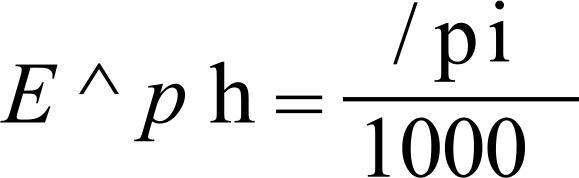
\includegraphics{0034-8910-rsp-48-01-0086-ii01}, sendo \textit{p}
\textit{i}
a proporção estimada na amostra\textit{ i}. O erro padrão do estimador foi calculado por:
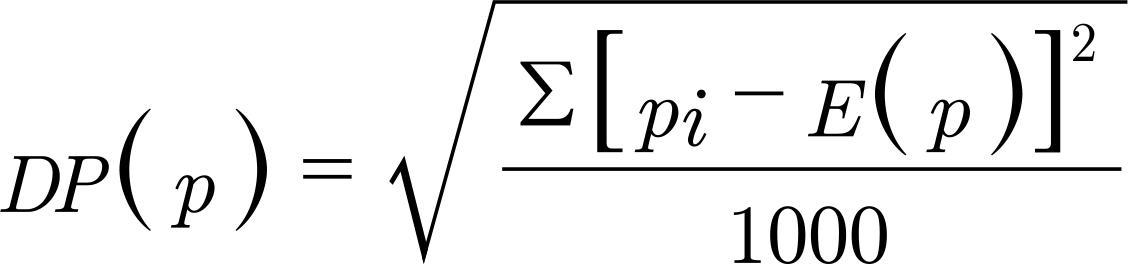
\includegraphics{0034-8910-rsp-48-01-0086-ii02}; o vício por: Vic(p)=E(p)-P, e o
erro quadrático médio, indicador da acurácia do estimador, por:
\textsc{eqm}(p)=[DP(p)]\textsuperscript{2}
+[Vic(p)]\textsuperscript{2}.

Os delineamentos de amostragem foram comparados por meio de medidas
relativas.\textsuperscript{[}\textsuperscript{10}\textsuperscript{]}\textsuperscript{,}\textsuperscript{[}\textsuperscript{12}\textsuperscript{]}
A precisão foi comparada pelo coeficiente de variação
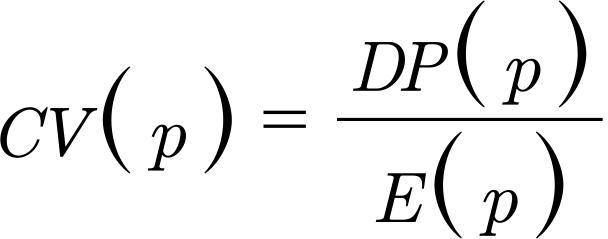
\includegraphics{0034-8910-rsp-48-01-0086-ii03}, o vício por meio do vício
relativo (razão entre o vício e a
média)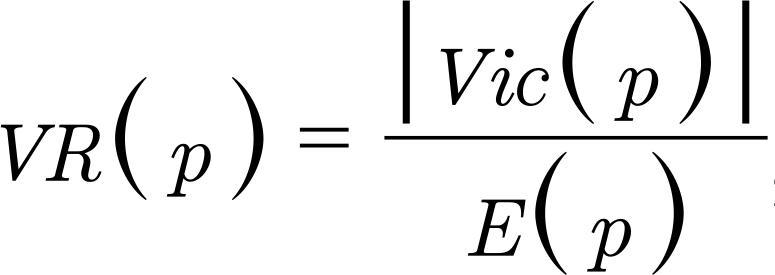
\includegraphics{0034-8910-rsp-48-01-0086-ii04} e a acurácia por meio do
erro quadrático médio relativo, 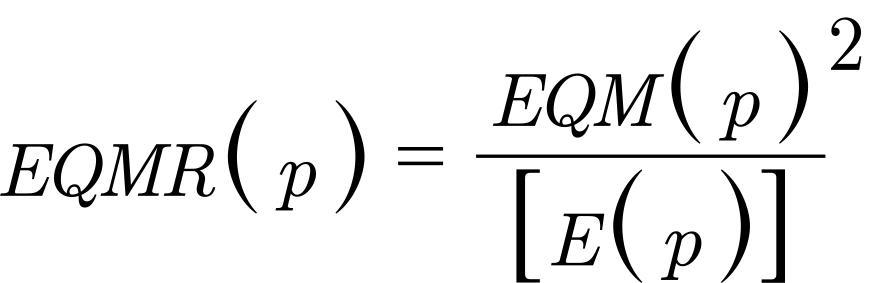
\includegraphics{0034-8910-rsp-48-01-0086-ii05}.
Para detectar o impacto do vício nas inferências por intervalo de confiança, foi
empregada a razão entre o vício e o erro padrão

\includegraphics{0034-8910-rsp-48-01-0086-ii06}, adotando critério proposto por
Cochran.\textsuperscript{[}\textsuperscript{6}\textsuperscript{]}
Se o vício for menor que a décima parte do erro padrão da estimativa (razão
menor que 0,10), será considerado desprezível.

Considerou-se que a eficiência de um delineamento diz respeito ao grau de
adequação entre as exigências de precisão e vício das estimativas e o custo de
obtê-las. Kish\textsuperscript{[}\textsuperscript{10}\textsuperscript{]}
propõe que a comparação entre o custo dos delineamentos com sorteio de uma única
pessoa e sem sorteio intradomiciliar seja feita pela expressão: custo = nc +
m.dc, em que \textit{c}
é o custo básico por elemento (pessoa), igual para os dois delineamentos, tais
como: aplicação de questionários e processamento de dados; \textit{dc}
é o custo de incluir um domicílio, tais como: custo de pedir permissão para
entrar no domicílio, de conseguir cooperação dos moradores e de realizar a
listagem de moradores; \textit{n}
é número de pessoas e \textit{m}
é o número de domicílios.

\section{\textsc{resultados}}

Foram inicialmente calculadas as proporções populacionais para as variáveis do
estudo e as médias das estimativas obtidas sob os dois delineamentos em
avaliação, com e sem sorteio intradomiciliar, para os dois grupos populacionais
de interesse, adultos e o conjunto de adultos e idosos (Tabela 2).

Tabela 2Parâmetros para proporções (P) de adultos e de adultos/idosos e médias
das distribuições de frequência [E(p)], segundo delineamento com sorteio (del1)
e sem sorteio (del2). Região Metropolitana da Baixada Santista, SP, 2006-2007.
\begin{table}
\begin{xtabular}{ l | l | l l | l }
\hline
Proporções & P & E(p) \\ \hline
del1 & del2\\ \hline
\multirow{1}{*}{\multicolumn{2}{l}{Adultos}}
&
&
\\ \hline

& Possui 8 ou mais bens domésticos
& 46,237
& 46,128
& 46,344
\\ \hline

& Auto avaliação ruim
& 10,755
& 10,806
& 10,752
\\ \hline

& Deixou de realizar atividade nos últimos 15 dias
& 13,177
& 13,197
& 13,175
\\ \hline

& Refere hipertensão
& 17,637
& 17,632
& 17,612
\\ \hline

& Tomou medicamentos para HA nos últimos 15 dias
& 70,781
& 70,799
& 70,921
\\ \hline

& Refere diabetes
& 4,805
& 4,814
& 4,798
\\ \hline

& Possui convenio ou plano de saúde
& 42,313
& 42,273
& 42,394
\\ \hline

& Precisou de atendimento de saúde nos últimos 15dias
& 19,374
& 19,434
& 19,322
\\ \hline

& Foi receitado algum medicamento nesse atendimento
& 59,429
& 59,440
& 59,294
\\ \hline

& Consulta odontológica no último ano
& 44,304
& 44,207
& 44,353
\\ \hline

\multirow{1}{*}{\multicolumn{2}{l}{Adultos e idosos}}
&
&
\\ \hline

& Possui 8 ou mais bens domésticos
& 46,472
& 46,326
& 46,275
\\ \hline

& Auto avaliação ruim
& 13,228
& 13,236
& 13,185
\\ \hline

& Deixou de realizar atividade nos últimos 15 dias
& 13,476
& 13,562
& 13,321
\\ \hline

& Refere hipertensão
& 22,698
& 22,617
& 22,567
\\ \hline

& Tomou medicamentos para HA nos últimos 15 dias
& 78,026
& 77,898
& 78,284
\\ \hline

& Refere diabetes
& 7,286
& 7,286
& 7,256
\\ \hline

& Possui convênio ou plano de saúde
& 43,267
& 43,331
& 43,344
\\ \hline

& Precisou de atendimento de saúde nos últimos 15dias
& 20,093
& 20,199
& 20,046
\\ \hline

& Foi receitado algum medicamento nesse atendimento
& 57,638
& 57,435
& 57,185
\\ \hline

& Consulta odontológica no último ano
& 41,808
& 41,857
& 41,880
\\ \hline

\end{xtabular}
\end{table}

HA: Hipertensão arterial

HA: Hipertensão arterial

As diferenças entre a esperança do estimador \textit{p}
e o parâmetro populacional, equivalente ao vício do estimador, foram semelhantes
para os dois delineamentos. Isso pode ser atestado pela proximidade das
estimativas do vício relativo. As diferenças, à exceção de uma delas,
situaram-se na terceira casa decimal (Tabela 3). As razões entre o vício e o
erro padrão foram menores que 0,10, indicando vícios desprezíveis para ambos os
delineamentos.

Tabela 3Razões vício/média e vício/erro, segundo delineamento de amostragem com
sorteio (del1) e sem sorteio (del2). Região Metropolitana da Baixada Santista,
SP, 2006-2007.
\begin{table}
\begin{xtabular}{ l | l | l l | l | l | l }
\hline
Estimadores & Vício/média & Vício/erro\\ \hline
\\ \hline
del1 & del2 & del1 & del2\\ \hline
\multirow{1}{*}{\multicolumn{2}{l}{Adultos}}
&
&
&
\\ \hline

& Possui 8 ou mais bens domésticos
& 0,0024
& 0,0023
& 0,034
& 0,027
\\ \hline

& Auto avaliação ruim
& 0,0048
& 0,0002
& 0,034
& 0,002
\\ \hline

& Deixou de realizar atividade nos últimos 15 dias
& 0,0015
& 0,0002
& 0,012
& 0,001
\\ \hline

& Refere hipertensão
& 0,0003
& 0,0014
& 0,003
& 0,015
\\ \hline

& Tomou medicamentos para HA nos últimos 15 dias
& 0,0003
& 0,0020
& 0,003
& 0,028
\\ \hline

& Refere diabetes
& 0,0019
& 0,0015
& 0,008
& 0,007
\\ \hline

& Possui convenio ou plano de saúde
& 0,0009
& 0,0019
& 0,014
& 0,025
\\ \hline

& Precisou de atendimento de saúde nos últimos 15dias
& 0,0031
& 0,0027
& 0,030
& 0,029
\\ \hline

& Foi receitado algum medicamento nesse atendimento
& 0,0002
& 0,0023
& 0,002
& 0,027
\\ \hline

& Consulta odontológica no último ano
& 0,0022
& 0,0011
& 0,038
& 0,019
\\ \hline

\multirow{1}{*}{\multicolumn{2}{l}{Adultos e idosos}}
&
&
&
\\ \hline

& Possui 8 ou mais bens domésticos
& 0,0031
& 0,0043
& 0,046
& 0,049
\\ \hline

& Auto avaliação ruim
& 0,0006
& 0,0033
& 0,005
& 0,027
\\ \hline

& Deixou de realizar atividade nos últimos 15 dias
& 0,0064
& 0,0116
& 0,052
& 0,097
\\ \hline

& Refere hipertensão
& 0,0036
& 0,0058
& 0,038
& 0,066
\\ \hline

& Tomou medicamentos para HA nos últimos 15 dias
& 0,0016
& 0,0033
& 0,030
& 0,064
\\ \hline

& Refere diabetes
& 0,0001
& 0,0041
& 0,000
& 0,024
\\ \hline

& Possui convênio ou plano de saúde
& 0,0015
& 0,0018
& 0,022
& 0,022
\\ \hline

& Precisou de atendimento de saúde nos últimos 15dias
& 0,0052
& 0,0023
& 0,051
& 0,025
\\ \hline

& Foi receitado algum medicamento nesse atendimento
& 0,0035
& 0,0079
& 0,034
& 0,086
\\ \hline

& Consulta odontológica no último ano
& 0,0012
& 0,0017
& 0,019
& 0,029
\\ \hline

\end{xtabular}
\end{table}

HA: Hipertensão arterial

HA: Hipertensão arterial

A comparação entre os coeficientes de variação indica que existência de sorteio
intradomiciliar levou a aumento do erro de amostragem para a maior parte das
variáveis (Tabela 4). Esse resultado se reflete nas medidas de acurácia. Para
80,0\% das variáveis, as estimativas do erro quadrático médio relativo foram
inferiores no delineamento sem sorteio nos domicílios.

Tabela 4Coeficiente de variação [CV(p)] e erro quadrático médio relativo
[\textsc{eqmr}(p)], segundo delineamento de amostragem com sorteio (del1) e sem sorteio
(del2). Região Metropolitana da Baixada Santista, SP, 2006-2007.
\begin{table}
\begin{xtabular}{ l | l | l l | l | l | l }
\hline
Estimadores & CV (p) & \textsc{eqmr} (p)\\ \hline
\\ \hline
del1 & del2 & del1 & del2\\ \hline
\multirow{1}{*}{\multicolumn{2}{l}{Adultos}}
&
&
&
\\ \hline

& Possui 8 ou mais bens domésticos
& 6,902
& 8,642
& 0,005
& 0,007
\\ \hline

& Auto avaliação ruim
& 14,200
& 13,336
& 0,020
& 0,018
\\ \hline

& Deixou de realizar atividade nos últimos 15 dias
& 12,823
& 10,996
& 0,016
& 0,012
\\ \hline

& Refere hipertensão
& 11,040
& 9,519
& 0,012
& 0,009
\\ \hline

& Tomou medicamentos para hipertensão arterial nos últimos 15 dias
& 7,496
& 7,000
& 0,006
& 0,005
\\ \hline

& Refere diabetes
& 24,610
& 21,606
& 0,061
& 0,047
\\ \hline

& Possui convênio ou plano de saúde
& 6,606
& 7,647
& 0,004
& 0,006
\\ \hline

& Precisou de atendimento de saúde nos últimos 15dias
& 10,238
& 9,267
& 0,010
& 0,009
\\ \hline

& Foi receitado algum medicamento nesse atendimento
& 9,849
& 8,594
& 0,010
& 0,007
\\ \hline

& Consulta odontológica no último ano
& 5,715
& 5,697
& 0,003
& 0,003
\\ \hline

\multirow{1}{*}{\multicolumn{2}{l}{Adultos e idosos}}
&
&
&
\\ \hline

& Possui 8 ou mais bens domésticos
& 6,846
& 8,638
& 0,005
& 0,007
\\ \hline

& Auto avaliação ruim
& 12,267
& 12,132
& 0,015
& 0,015
\\ \hline

& Deixou de realizar atividade nos últimos 15 dias
& 12,231
& 12,004
& 0,015
& 0,015
\\ \hline

& Refere hipertensão
& 9,333
& 8,838
& 0,009
& 0,008
\\ \hline

& Tomou medicamentos para hipertensão arterial nos últimos 15 dias
& 5,502
& 5,159
& 0,003
& 0,003
\\ \hline

& Refere diabetes
& 19,736
& 17,182
& 0,039
& 0,030
\\ \hline

& Possui convênio ou plano de saúde
& 6,760
& 7,933
& 0,005
& 0,006
\\ \hline

& Precisou de atendimento de saúde nos últimos 15dias
& 10,292
& 9,228
& 0,011
& 0,009
\\ \hline

& Foi receitado algum medicamento nesse atendimento
& 10,330
& 9,223
& 0,011
& 0,009
\\ \hline

& Consulta odontológica no último ano
& 6,105
& 5,923
& 0,004
& 0,004
\\ \hline

\end{xtabular}
\end{table}

Em relação ao custo, considerando o número de pessoas incluídas na amostra nos
dois delineamentos, 480, e os números de domicílios: 480 no delineamento com
sorteio e 240 (para adultos) e 226 ou 227 (para adultos e idosos) no
delineamento sem sorteio, tem-se que os custos foram maiores para este último.
Para adultos, foram pesquisados 240 domicílios a mais; para adultos e idosos em
conjunto, 254 domicílios a mais.

\section{\textsc{discussão}}

Os resultados do presente estudo indicam que, nas condições em que as amostras
foram sorteadas, o delineamento que não prevê o sorteio dentro do domicílio é
superior em termos de acurácia ao que preconiza o sorteio de uma pessoa por
domicílio. Embora as diferenças não sejam grandes, o menor custo do primeiro
delineamento agrega mais uma vantagem, confirmando sua superioridade. Em geral,
um desenho ótimo é desenvolvido determinando o efeito no custo e na variância de
procedimentos alternativos de amostragem e escolhendo o que minimiza a variância
para um custo fixo.\textsuperscript{[}\textsuperscript{12}\textsuperscript{]}

Os números médios de adultos dentro dos domicílios e o de adultos e idosos, em
conjunto, foram baixos: 2 e 2,12, respectivamente. Nessa situação, a
concentração de entrevistas nos domicílios não é grande, o que favorece a opção
de não realizar o sorteio.\textsuperscript{[}\textsuperscript{10}\textsuperscript{]}
Isso ocorre em diversos inquéritos, tanto os que são dirigidos para grupos
populacionais específicos,\textsuperscript{[}\textsuperscript{3}\textsuperscript{]}\textsuperscript{,}\textsuperscript{[}\textsuperscript{17}\textsuperscript{]}
como os que definem domínios de idade ou
sexo.\textsuperscript{[}\textsuperscript{1}\textsuperscript{]}\textsuperscript{,}\textsuperscript{[}\textsuperscript{15}\textsuperscript{]}
Nestes, a homogeneidade intradomiciliar não é relevante uma vez que as análises
são conduzidas para grupos populacionais específicos e para os quais há,
geralmente, pequena aglomeração no nível
domiciliar.\textsuperscript{[}\textsuperscript{12}\textsuperscript{]}
Krenzke et al\textsuperscript{[}\textsuperscript{11}\textsuperscript{]}
confirmam que, quando há múltiplos domínios de interesse, é frequentemente
melhor entrevistar mais de uma pessoa dentro do domicílio.

O efeito de conglomerado é um dos fatores que aumenta a variância das
estimativas obtidas nos inquéritos. No entanto, para amostras em múltiplos
estágios, o impacto na variância da homogeneidade dentro dos domicílios é
afetado pela homogeneidade existente nas unidades de amostragem anteriores.
Assim sendo, o impacto incremental da conglomeração dentro de domicílios pode
ser amortecido pela dominação dos componentes de variância do primeiro estágio
de seleção.\textsuperscript{[}\textsuperscript{11}\textsuperscript{]}

No presente estudo, somente os dois indicadores para os quais eram esperados
valores iguais para os moradores de um mesmo domicílio (posse de plano de saúde
e número de bens no domicílio) apresentaram erros de amostragem maiores sob o
delineamento sem sorteio. Embora o estudo desses indicadores não se constitua
objeto de pesquisas na área de saúde, é possível supor que existam indicadores
“de saúde” para os quais a correlação intradomicílio seja extremamente alta,
como ocorre quando estimativas são exatamente iguais para todos os moradores dos
domicílios. Nessas situações, a superioridade do delineamento sem sorteio deixa
de existir.

Krenzke et al\textsuperscript{[}\textsuperscript{11}\textsuperscript{]}
avaliaram diversas regras de seleção referentes ao número de adultos sorteados
dentro dos domicílios em delineamentos de quatro estágios: sorteio de um adulto
independente do número existente; sorteio de um adulto se houver até dois e
sorteio de dois para mais adultos; sorteio de um adulto se houver até três e de
dois para mais adultos; sorteio de um adulto se houver até quatro e de dois para
mais adultos; e sorteio de um ou dois adultos, sendo o tamanho da amostra uma
fração. Os autores propuseram uma forma de computar o efeito do delineamento
devido à homogeneidade domiciliar. Mediram, então, a redução percentual da
função variância/custo para as várias estratégias propostas em relação à de “um
adulto sorteado” e verificaram que a homogeneidade domiciliar teve pequeno
impacto na redução dessa função. A função variância/custo levou em conta a
função custo proposta por Kish,\textsuperscript{[}\textsuperscript{10}\textsuperscript{]}
que inclui o custo de inclusão de uma pessoa e de um domicílio, e os efeitos de
delineamento devido à conglomeração e à ponderação. Mostraram, ainda, que a
redução foi fortemente influenciada pelo nível de dominação dos componentes de
variância dos dois primeiros estágios de seleção.

O efeito de conglomerado não é o único fator que aumenta a variância. Esse
aumento também pode ser causado pela utilização de pesos no cálculo das
estimativas, decorrente da seleção de indivíduos com probabilidades distintas
dentro dos domicílios. Por meio de pesos, cada observação feita na pessoa
sorteada é repetida tantas vezes quantas forem os moradores existentes no
domicílio, inflacionando o efeito do delineamento. Assim, a probabilidade de
seleção passa a depender do número de pessoas no domicílio e o aumento da
variância estará diretamente relacionado ao coeficiente de variação desses
tamanhos.\textsuperscript{[}\textsuperscript{11}\textsuperscript{]}
O efeito do delineamento total é, sob algumas condições, o produto do efeito do
delineamento devido ao sorteio de conglomerados e do efeito do delineamento
devido à ponderação dos dados.

Dentre os fatores que têm sido apontados como favoráveis ao sorteio
intradomiciliar inclui-se a possibilidade de que as taxas de respostas sejam
afetadas pela sobrecarga que os moradores podem sentir com a realização de
várias entrevistas no mesmo domicílio.\textsuperscript{[}\textsuperscript{4}\textsuperscript{]}
No entanto, estudos recentes têm mostrado resultados que contradizem essa
avaliação. Mohadjer et al\textsuperscript{[}\textsuperscript{12}\textsuperscript{]}
consideram que a seleção de amostras maiores dentro dos domicílios é uma
abordagem com impacto favorável nas taxas de resposta do \textit{National Health
and Nutrition Examination Survey}. Esse inquérito prevê a realização de exames sorológicos e torna-se conveniente
para os membros do domicílio ir juntos ao centro de exames. As taxas de resposta
para o delineamento sem sorteio foram superiores às obtidas com sorteio
(acréscimo de 3,8 a 6,9 pontos percentuais, dependendo do tipo de domicílio). Da
mesma forma, Krenzke et al\textsuperscript{[}\textsuperscript{11}\textsuperscript{]}
não observaram diferenças estatisticamente significantes nas taxas de resposta
obtidas sob delineamentos com sorteio de uma ou de duas pessoas por domicílio na
\textit{National Assessment of Adult Literacy}.

Há ainda outros fatores que podem ser levados em conta ao se optar pela
realização ou não do sorteio intradomicilar. Contrário ao sorteio está o
interesse no estudo da dependência entre valores para diferentes pessoas de um
mesmo domicílio.

A favor do sorteio, menciona-se a existência de perguntas sensíveis nos
questionários, cujas respostas podem ter a qualidade comprometida ao serem
respondidas por mais de uma pessoa do
domicílio.\textsuperscript{[}\textsuperscript{5}\textsuperscript{]}
Foreman\textsuperscript{[}\textsuperscript{7}\textsuperscript{]}
também aventa a possibilidade de que a reação à entrevista de um dos moradores
contamine a resposta de outros, especialmente quando as entrevistas são muito
longas ou desconfortáveis. Na mesma linha de argumentação,
Kish\textsuperscript{[}\textsuperscript{10}\textsuperscript{]}
afirma que um dos motivos para não realizar mais que uma entrevista por
domicílio é evitar que o respondente tenha oportunidade de discutir as questões
previamente.

No presente estudo, o custo foi representado pelo número de domicílios, uma vez
que o número de pessoas entrevistadas foi igual nos dois delineamentos
comparados. O custo de inclusão de um domicílio na amostra é considerado sempre
superior ao de inclusão de uma pessoa por envolver a realização da listagem de
todos os moradores e o deslocamento entre endereços, quando as entrevistas são
face-a-face. Esse deslocamento ocorre em diversos momentos do processo de coleta
de dados: identificação dos moradores dos domicílios, realização da entrevista,
retornos para reversão da não resposta, supervisão e controle de qualidade.

Em nosso estudo, a amostra de domicílios sob o delineamento sem sorteio foi
metade daquela obtida no delineamento com sorteio, mostrando-se, portanto, mais
econômica. Esse é um aspecto relevante a ser considerado nos inquéritos
domiciliares com entrevistas face-a-face realizados na área de saúde pública,
uma vez que a diminuição de gastos é alternativa sempre desejada.

Deve-se considerar, ainda, que o sorteio de pessoas dentro dos domicílios
aumenta a complexidade das amostras. É necessário treinar o entrevistador para
que, em campo, utilize procedimentos adequados de sorteio que evitem a
introdução de vícios. É necessário, ainda, que sejam utilizados pesos que
compensem as diferenças na probabilidade de seleção dos indivíduos da amostra,
produzidas pelo sorteio de um número fixo de moradores (um, em geral) na
presença de diferentes números de moradores. A não introdução desses pesos, como
não raro ocorre em análises de dados advindos de inquéritos que utilizam o
sorteio intradomiciliar, produz estimativas viciadas.

Os resultados deste estudo mostraram que o delineamento sem sorteio dentro do
domicílio é mais eficiente, devendo ser a opção preferencial do pesquisador. O
sorteio de moradores deve ser adotado quando houver razões referentes ao objeto
de estudo que possam levar à introdução de vícios nas respostas dos
entrevistados caso vários moradores respondam ao questionário proposto.

\section*{\textsc{referências}}
\begin{itemize}

\item[1] Bastos TF, Alves \textsc{mcgp}, Barros \textsc{mba}, Cesar \textsc{clg}. A saúde dos homens:
desigualdades sociais em estudo de base populacional. \textit{Cad Saude
Publica.}
2012;28(11):2133-42. \textsc{doi}:10.1590/S0102-311X2012001100013

\item[2] Berquó ES. Selección de unidades de información en encuestas
demográficas: un método para construir tablas de sorteio. Santiago: \textsc{celade}; 1975
(Notas de Población, 3).

\item[3] Berquó ES, Garcia S, Lima L. Reprodução na juventude: perfis
sociodemográficos, comportamentais e reprodutivos na \textsc{pnds} 2006. \textit{Rev
Saude Publica. }
2012;46(4):685-93. \textsc{doi}:10.1590/S0034-89102012005000048

\item[4] Clark RG, Steel DG. Sampling within households in household surveys.
\textit{J Royal Statist Soc Series A.}
2007;170(1):63-82. \textsc{doi}:10.1111/j.1467-985X.2006.00434.x

\item[5] Clark RG, Steel DG. The effect of using household as a sampling unit.
\textit{Int Statist Rev}. 2002;70(2):289-314.

\item[6] Cochran WG. Sampling techniques. 3. ed. New York: John Wiley \& Sons;
1977.

\item[7] Foreman E. Survey sampling principles. New York: Marcel Dekker; 1991.

\item[8] Kish L, Frankel MR. Inference from complex samples. \textit{J Rl Stat
Soc. Series B Stat Methodol.}
1974;36:1-37.

\item[9] Kish L. A procedure for objetive respondent selection within the
household. \textit{Amer Statist Assoc J.}
1949;44(247):380-7. \textsc{doi}:10.1080/01621459.1949.10483314

\item[10] Kish L. Survey sampling. New York: John Wiley \& Sons; 1965.

\item[11] Krenzkle T, Li L, Rust K. Evaluating within household selection rules
under a multi-stage design. \textit{Surv Methodol.}
2010;36(1):111-9.

\item[12] Mohadjer L, Curtin LR. N. Balancing sample design goals for the
National Health and Nutrition Examination Survey. \textit{Surv Methodol. }
2008;34(1):119-26.

\item[13] O’Rourke D, Blair J. Improving random respondent selection in
telephone surveys. \textit{J Marketing Res.}
1983;20(4):428-32.

\item[14] Oldendick RW, Bishop GF, Sorenson SB, Tuchfarber AJ. A comparison of
the Kish and last birthday methods of respondent selection in telephone surveys.
\textit{J Official Statist.}
1988;4(4):307-18.

\item[15] Roncalli AG, Silva NN, Nascimento AC, Freitas \textsc{chsm}, Casotti E, Peres
KG, et al. Aspectos metodológicos do Projeto \textsc{sbb}rasil 2010 de interesse para
inquéritos nacionais de saúde. \textit{Cad Saude Publica.}
2012;28Suppl:40-57. \textsc{doi}:10.1590/S0102-311X2012001300006

\item[16] Salmon CT, Nichols JS. The next-birthday method of respondent
selection. \textit{Public Opinion Q.}
1983;47(2):270-6. \textsc{doi}:10.1086/268785

\item[17] Silva NN. Processo de amostragem. In: Lebrão ML, Duarte \textsc{yao}. O projeto
\textsc{sabe} no Município de São Paulo: uma abordagem inicial. Brasília (DF):
Organização Pan-Americana da Saúde; 2003.

\end{itemize}

\end{document}
